\task{Поделим – посмотрим}
\begin{itemize}

\itA Пусть даны два прямоугольных треугольника. Каждая сторона первого из них может пересекать второй треугольник не более чем дважды, в сиду выпуклости прямоугольного треугольника. Значит, два прямоугольных треугольника могут иметь не более шести пересечений (причем шесть пересечений получить можно — достаточно взглянуть на «звезду Давида»).

Заметим теперь, что для замкнутой линии количество областей, которые она добавляет к картинке, равно количеству ее пересечений с другими, уже имеющимися, линиями.

Первый треугольник делит плоскость на две области. Второй, пересекаясь с ним максимум 6 раз, добавит еще шесть областей. Третий треугольник может не более чем по шесть раз пересечь первые два, то же верно и про четвертый треугольник.

Отсюда мы получаем верхнюю оценку на количество областей:
$$2 + 6 + 6 \cdot 2 + 6 \cdot 3 = 38.$$

Мы уже доказали, что больше 38 областей получить нельзя — в свою очередь, получить ровно 38 можно, для этого расположим треугольники «достаточно хаотично»:

\begin{center}
	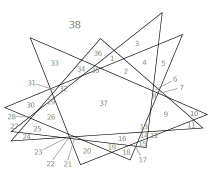
\includegraphics[width=7.5cm]{figures/2017-5-1a}
\end{center}

\itB Прямая может «входить» в семиугольник и «выходить» из него. При этом изначально она находится снаружи и в конце должна оказаться там же. Каждую сторону семиугольника прямая пересекает не более одного раза, а количество пересечений должно быть четным. Значит, прямая пересекает максимум шесть сторон, «проходя» через семиугольник трижды.

Получается, она делит семиугольник на максимум на четыре части: до первого пересечения, между первым и вторым, между вторым и третьим, после третьего пересечения.

\itC Два одинаково ориентированных квадрата пересекаются максимум в двух точках (если не совпадают). Это значит, что $k$--ый нарисованный квадрат добавляет на картинку не более $2(k-1)$ новых областей. Отсюда ответ на задачу — $2+2+4+\ldots+2\cdot 14$ $=$ $2+2\cdot105$ $=$ $312$.

Изобразить 15 попарно пересекающихся квадратов несложно — достаточно взять один и 14 раз немного сдвинуть его по диагонали.
\end{itemize}